\chapter{DESENVOLVIMENTO DO PROJETO}
%\section{Escopo do Projeto}
%\subsection{Regras de Negócio}
%\subsection{Requisitos Funcionais}
%\subsection{Requisitos Não Funcionais}
%
\section{Escopo do Projeto}
O escopo do projeto define os limites, objetivos e funcionalidades do sistema desenvolvido. Nesta etapa, são apresentadas as regras de negócio, os requisitos funcionais e não funcionais que orientam o desenvolvimento da aplicação. Esses elementos determinam o que será implementado e asseguram que o sistema atenda de forma precisa às necessidades da loja \textbf{Tropical Mix}.


\subsection{Regras de Negócio}

A Tabela~\ref{tab:regras-negocio} apresenta as regras de negócio estabelecidas para o sistema web da loja \textbf{Tropical Mix}. Essas regras foram definidas para garantir o controle, a integridade e a padronização dos processos internos relacionados à gestão de estoque e vendas.

\begin{table}[H]
\centering
\caption{Regras de Negócio}
\label{tab:regras-negocio}
\begin{tabular}{|p{2cm}|p{3cm}|p{4cm}|p{6.5cm}|}
\hline
\textbf{Código} & \textbf{Atores} & \textbf{Nome da Regra} & \textbf{Descrição} \\ \hline
RN01 & Administrador & Permissão de Acesso & Somente usuários autenticados podem acessar o sistema. Perfis diferentes (administrador e funcionário) possuem permissões distintas de visualização e edição de dados. \\ \hline
RN02 & Administrador & Controle de Estoque Automático & O sistema deve atualizar automaticamente o estoque a cada venda registrada ou movimentação de entrada/saída de produtos, garantindo integridade das informações. \\ \hline
RN03 & Funcionário & Registro Obrigatório de Vendas & Nenhuma venda pode ser finalizada sem que todos os campos obrigatórios estejam preenchidos: produto, quantidade, preço e forma de pagamento. \\ \hline
RN04 & Administrador & Bloqueio de Exclusão de Produto & Produtos associados a vendas registradas não podem ser excluídos do sistema. Nesses casos, apenas a desativação do item será permitida, mantendo o histórico de dados. \\ \hline
RN05 & Administrador / Funcionário & Alerta de Reposição & O sistema deverá emitir alertas automáticos para o administrador quando a quantidade de determinado produto atingir o nível mínimo definido para reposição de estoque. \\ \hline
RN06 & Administrador & Relatórios Consolidados & Relatórios gerenciais devem consolidar dados de vendas, estoque e movimentações, apresentando indicadores de desempenho e tendências em períodos configuráveis. \\ \hline
RN07 & Administrador & Registro de Ações & Toda ação administrativa relevante (cadastro, alteração ou exclusão) deve ser registrada em log interno, permitindo rastreabilidade e auditoria de operações. \\ \hline
\end{tabular}
\fonte{Elaborado pelos autores.}
\end{table}

\vspace{-0.5cm} % reduz espaço vertical entre tabelas

\subsection{Requisitos Funcionais}

A Tabela~\ref{tab:requisitos-funcionais} apresenta os requisitos funcionais do sistema, os quais descrevem as funcionalidades que devem ser implementadas para atender às regras de negócio e às necessidades operacionais da loja \textbf{Tropical Mix}.

\begin{table}[H]
\centering
\caption{Requisitos Funcionais do Sistema}
\label{tab:requisitos-funcionais}
\begin{tabular}{|p{2cm}|p{3cm}|p{3.5cm}|p{7cm}|}
\hline
\textbf{Código Requisito} & \textbf{Atores} & \textbf{Nome} & \textbf{Descrição} \\ \hline
RF01 & Administrador & Cadastro de Produtos & O sistema deve permitir que o administrador cadastre novos produtos no estoque, informando nome, categoria, quantidade, preço de venda e data de inclusão. Cada produto deve possuir um identificador único e poderá ser atualizado ou desativado posteriormente. \\ \hline
RF02 & Administrador / Funcionário & Controle de Estoque & A aplicação deverá permitir o controle de entrada e saída de produtos, atualizando automaticamente a quantidade em estoque a cada movimentação registrada. O sistema deverá alertar quando um item atingir o nível mínimo definido para reposição. \\ \hline
RF03 & Funcionário & Registro de Vendas & O sistema deve possibilitar o registro de vendas, vinculando cada operação a um funcionário responsável e à data da transação. As vendas devem reduzir automaticamente o estoque e gerar recibos ou relatórios para conferência. \\ \hline
RF04 & Administrador & Relatórios Gerenciais & A aplicação deverá permitir a geração de relatórios personalizados sobre movimentações de estoque, volume de vendas, produtos mais vendidos e desempenho por período. Esses relatórios deverão ser exibidos em formato gráfico e exportáveis em PDF. \\ \hline
RF05 & Administrador / Funcionário & Autenticação de Usuário & O sistema deve conter uma tela de login, permitindo o acesso apenas a usuários cadastrados. Perfis de acesso devem ser diferenciados entre administradores e funcionários, restringindo funções conforme as permissões atribuídas. \\ \hline
RF06 & Administrador & Gerenciamento de Usuários & O administrador deverá ser capaz de cadastrar, editar ou excluir usuários do sistema, definindo perfis e senhas de acesso. Cada alteração deverá ser registrada para fins de auditoria e segurança. \\ \hline
RF07 & Administrador & Dashboard Dinâmico & A aplicação deve conter um painel de controle (Dashboard) que apresente informações atualizadas em tempo real, como faturamento diário, produtos com menor estoque e histórico de vendas mensais. \\ \hline
\end{tabular}
\fonte{Elaborado pelos autores.}
\end{table}

\vspace{-0.5cm}

\subsection{Requisitos Não Funcionais}

A Tabela~\ref{tab:requisitos-nao-funcionais} apresenta os requisitos não funcionais definidos para o sistema web da loja \textbf{Tropical Mix}. Esses requisitos descrevem as propriedades de qualidade e desempenho que o sistema deve atender, garantindo segurança, usabilidade e confiabilidade nas operações realizadas.

\begin{table}[H]
\centering
\caption{Requisitos Não Funcionais do Sistema}
\label{tab:requisitos-nao-funcionais}
\begin{tabular}{|p{2cm}|p{3cm}|p{4cm}|p{6.5cm}|}
\hline
\textbf{Código} & \textbf{Categoria} & \textbf{Nome do Requisito} & \textbf{Descrição} \\ \hline

RNF01 & Desempenho & Tempo de Resposta & 
O sistema deve responder às requisições do usuário em até 3 segundos, mesmo durante picos de acesso. \\ \hline

RNF02 & Usabilidade & Interface Intuitiva & 
A interface deve ser simples e de fácil navegação, permitindo que usuários sem experiência técnica realizem as principais tarefas de forma autônoma. \\ \hline

RNF03 & Segurança & Controle de Acesso & 
O sistema deve garantir autenticação de usuários com senhas criptografadas e níveis de permissão definidos conforme o perfil (administrador ou funcionário). \\ \hline

RNF04 & Confiabilidade & Backup Automático & 
Os dados do sistema devem ser salvos automaticamente em cópias de segurança diárias, evitando perda de informações em caso de falha. \\ \hline

RNF06 & Manutenibilidade & Código Modular e Documentado & 
O sistema deve ser desenvolvido em arquitetura modular, com código documentado, facilitando futuras atualizações e manutenção técnica. \\ \hline

RNF07 & Disponibilidade & Funcionamento Contínuo & 
O sistema deve estar disponível 99\% do tempo, com exceção de períodos programados de manutenção. \\ \hline

\end{tabular}
\fonte{Elaborado pelos autores.}
\end{table}




%\section{Histórias de Usuário}
%\subsection{Descrição das Histórias}
\section{Histórias de Usuário}
\subsection{Descrição das Histórias}

%\section{Arquitetura} % FEITO
%\subsection{Definições da Arquitetura} % FEITO
%\subsection{Diagrama da Arquitetura} % FEITO
\section{Arquitetura}

\subsection{Definição da Arquitetura}

A arquitetura proposta para o sistema web da loja \textbf{Tropical Mix} baseia-se em um modelo multicamadas, que separa claramente a interface de apresentação (\textit{front-end}), a lógica de negócio (\textit{back-end}) e o armazenamento de dados (banco de dados). Essa abordagem visa garantir modularidade, escalabilidade e facilidade de manutenção, além de permitir futuras expansões do sistema.

No nível de apresentação, o \textit{front-end} foi desenvolvido utilizando a biblioteca \textbf{React}, em conjunto com \textbf{JavaScript} e \textbf{HTML/CSS}. Essa combinação possibilita a criação de uma interface moderna, interativa e responsiva, permitindo que o sistema seja acessado por diversas pessoas.

Na camada de aplicação, responsável pela lógica de negócio, foi adotada a linguagem \textbf{Python} juntamente com o framework \textbf{Flask}. Essa tecnologia foi escolhida por oferecer leveza, flexibilidade e facilidade de integração com outras ferramentas, além de possuir uma ampla comunidade de suporte.

Para o gerenciamento e persistência de dados, o sistema utiliza o \textbf{MySQL} como banco de dados relacional. Essa escolha se deve à sua robustez, confiabilidade e compatibilidade com aplicações web modernas.

Além disso, a comunicação entre o \textit{front-end} e o \textit{back-end} é realizada via \textbf{API REST}, utilizando o formato \textbf{JSON} para o envio e recebimento de dados. Essa arquitetura baseada em serviços favorece a escalabilidade do sistema, permitindo que novas funcionalidades ou módulos possam ser integrados sem comprometer a estrutura existente.

\subsection{Diagrama da Arquitetura}

A Figura~\ref{fig:arquitetura} apresenta o diagrama de implantação do sistema, ilustrando a interação entre as camadas e os principais componentes que compõem a aplicação web.

\begin{figure}[H]
    \centering
    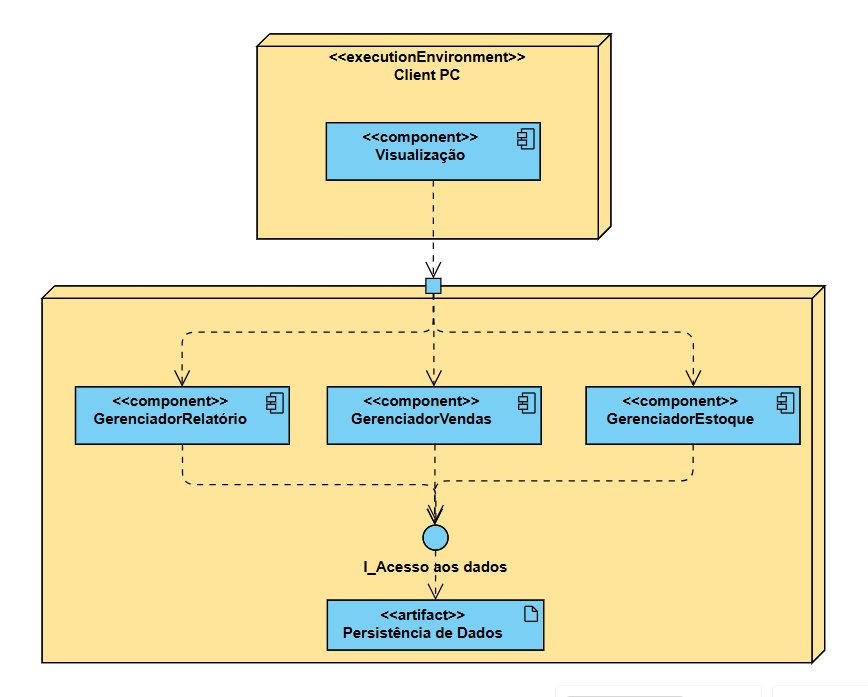
\includegraphics[width=0.9\textwidth]{LaTex/Capítulos/img/Desenvolvimento do Projeto/Arquitetura/arquitetura.png}
    \caption{Diagrama de Implantação}
    \fonte{Elaborado pelos autores.}
    \label{fig:arquitetura}
\end{figure}

Opcionalmente, a Figura~\ref{fig:componentes} apresenta o diagrama de componentes, que detalha a estrutura lógica do sistema e as dependências entre os módulos internos.

\begin{figure}[H]
  \centering
  \includegraphics[width=0.9\textwidth]{LaTex/Capítulos/img/Desenvolvimento do Projeto/Arquitetura/Diagrama_componentes.png}
  \caption{Diagrama de Componentes.}
  \fonte{Elaborado pelos autores.}
  \label{fig:componentes}
\end{figure}







%\section{Tecnologias}
\section{Tecnologias}

O desenvolvimento do sistema \textbf{Tropical Mix} foi estruturado a partir de um conjunto de tecnologias modernas e amplamente utilizadas no mercado de desenvolvimento web. A escolha das ferramentas considerou critérios como desempenho, escalabilidade, segurança e facilidade de manutenção. A seguir, são descritas as principais tecnologias aplicadas em cada camada da aplicação.

\subsection{Front-end}

A camada de \textit{front-end} do sistema foi desenvolvida utilizando a biblioteca \textbf{React.js}, que possibilita a criação de interfaces de usuário modernas, dinâmicas e responsivas. Essa tecnologia, baseada em componentes reutilizáveis, permite a construção de telas interativas e modulares, facilitando a manutenção e a evolução da aplicação.  

A escolha pelo React deve-se à sua eficiência no gerenciamento do estado da aplicação, à sua capacidade de atualização em tempo real e à ampla comunidade de desenvolvedores, o que assegura suporte contínuo e uma vasta gama de bibliotecas complementares.  

Para a estruturação e estilização das páginas, foram utilizadas as tecnologias \textbf{HTML5} e \textbf{CSS3}, permitindo a criação de layouts responsivos que se adaptam a diferentes dispositivos, como computadores, tablets e smartphones. A comunicação entre o \textit{front-end} e o \textit{back-end} é realizada por meio de requisições HTTP utilizando a biblioteca \textbf{Axios}, que possibilita a troca de dados de forma assíncrona e eficiente.  

Além das funcionalidades de navegação e controle de estoque e vendas, o \textit{front-end} também inclui o módulo de um painel dinâmico, \textbf{Dashboard}, um painel interativo voltado à geração de relatórios e à exibição de indicadores de desempenho. Esse painel consome dados disponibilizados pela API do \textit{back-end} e apresenta informações estratégicas, como volume de vendas, produtos com menor estoque e desempenho por período, em gráficos e tabelas dinâmicas.  

Dessa forma, o \textit{front-end} não apenas oferece uma interface intuitiva e agradável ao usuário, mas também serve como ferramenta de apoio à gestão, centralizando visualmente as informações mais relevantes para a tomada de decisão.

\subsection{Back-end}

O \textit{back-end} foi implementado utilizando a linguagem \textbf{Python}, em conjunto com o microframework \textbf{Flask}, responsável por gerenciar as rotas, processar as regras de negócio e realizar a comunicação com o banco de dados. O Flask foi escolhido por sua leveza, flexibilidade e fácil integração com outras tecnologias, além de oferecer suporte nativo à construção de APIs RESTful.  

Entre as principais funcionalidades desenvolvidas nessa camada, destacam-se:
\begin{itemize}
    \item Gerenciamento de usuários e autenticação, com controle de perfis de acesso;
    \item Registro e controle de vendas e movimentações de estoque;
    \item Processamento de dados para geração de relatórios e indicadores exibidos no painel do \textit{front-end};
    \item Integração com o banco de dados \textbf{MySQL} para armazenamento e consulta das informações.
\end{itemize}

O uso do Flask proporciona um desenvolvimento ágil, modular e seguro, permitindo que novas funcionalidades sejam incorporadas de forma independente, sem comprometer a arquitetura do sistema. A comunicação com o \textit{front-end} ocorre por meio de uma \textbf{API REST}, garantindo a troca estruturada e eficiente de dados no formato \textbf{JSON}.


\subsection{Banco de Dados}

O banco de dados escolhido para o sistema é o \textbf{MySQL}, um dos gerenciadores de banco de dados relacionais mais consolidados no mercado. Sua escolha foi motivada pela confiabilidade, escalabilidade e ampla compatibilidade com aplicações baseadas em Python.  

O modelo de dados foi projetado de forma a garantir integridade referencial e desempenho nas operações de leitura e escrita. Cada transação, seja de venda, compra ou atualização de estoque, é registrada no banco de dados, permitindo o acompanhamento detalhado das atividades da loja.  

Além disso, a estrutura relacional do MySQL possibilita consultas otimizadas para a geração de relatórios, facilitando a análise de dados e o processo de tomada de decisão por parte da gestão da \textbf{Tropical Mix}.



\subsection{Infraestrutura}

TEREMOS NÉ?


\subsection{Ferramentas de apoio}

TERAÁ ????
%\subsection{Front-end}
%\subsection{Back-end}
%\subsection{Banco de Dados}
%\subsection{Infraestrutura}


\section{Testes e Manutenibilidade}

A etapa de testes é planejada para assegurar a qualidade, a estabilidade e a confiabilidade do sistema em todas as suas camadas. O processo será conduzido em ambiente de desenvolvimento controlado, com o objetivo de identificar erros, validar funcionalidades e garantir que o comportamento da aplicação esteja de acordo com os requisitos definidos.

\subsection{Plano de Testes}

O plano de testes define os tipos, ferramentas e critérios que serão utilizados para verificar o funcionamento do sistema. Os principais módulos contemplados serão autenticação de usuários, controle de estoque, registro de vendas e geração de relatórios. Cada caso de teste será estruturado a partir de cenários reais de uso, assegurando que o sistema responda corretamente a diferentes condições e entradas de dados.

\subsection{Testes Funcionais}

Os testes funcionais têm como propósito validar se cada funcionalidade implementada cumpre as regras de negócio e os requisitos definidos. Essa categoria incluirá a verificação de rotas da API, formulários de entrada de dados e respostas esperadas na interface, garantindo que o sistema opere de forma coerente entre as camadas.

\subsubsection{Testes Unitários}

Os testes unitários serão aplicados à camada de back-end, utilizando a biblioteca \textbf{Pytest} para o framework Flask. Eles validarão funções individuais, como cadastro e atualização de produtos, autenticação e cálculos de estoque. O foco será garantir que cada parte do código funcione de forma independente e confiável.

\subsubsection{Testes de Integração}

Os testes de integração validarão o fluxo completo entre front-end, back-end e banco de dados. Serão simuladas requisições enviadas pelo React via Axios e processadas pelo Flask, com persistência no MySQL. Essa etapa confirmará a correta comunicação entre as camadas e o retorno de dados consistentes.

\subsubsection{Testes End-to-End}

Os testes end-to-end (\textit{E2E}) simularão a experiência completa do usuário no sistema, desde o login até o registro de uma venda e a atualização automática do estoque. Ferramentas como \textbf{Cypress} ou \textbf{Selenium} poderão ser utilizadas para automatizar esses fluxos, garantindo que as principais funcionalidades se comportem conforme o esperado em ambiente de execução real.

\subsection{Testes Não Funcionais}

Os testes não funcionais avaliarão aspectos de desempenho, segurança e confiabilidade da aplicação. Essa categoria inclui os seguintes subtipos:

\subsubsection{Testes de Performance}

Medirão o tempo de resposta das operações críticas, como consultas de estoque e geração de relatórios. O objetivo é garantir que as requisições sejam processadas em até 3 segundos, mesmo sob múltiplos acessos simultâneos.

\subsubsection{Testes de Carga}

Os testes de carga simularão múltiplos acessos simultâneos à aplicação, avaliando o comportamento do servidor e do banco de dados sob picos de utilização. Essa análise ajudará a identificar possíveis gargalos e a otimizar o uso de recursos.

\subsection{Logs e Manutenibilidade}

O sistema contará com logs automáticos integrados ao back-end, registrando operações críticas como cadastros, exclusões e alterações de dados. Esses registros serão essenciais para auditoria, depuração e rastreamento de falhas. 

A manutenibilidade será garantida pela adoção de código modular, documentação interna e versionamento contínuo no GitHub. Essas práticas permitirão a expansão do sistema e a correção de falhas de forma ágil e organizada.


\subsection{Code Convention}

As convenções de código adotadas no desenvolvimento do sistema \textbf{Tropical Mix} têm como finalidade garantir padronização, legibilidade e facilidade de manutenção do código. O uso de boas práticas de escrita e organização permite que o projeto seja compreendido por diferentes desenvolvedores, facilite futuras atualizações e reduza a ocorrência de erros.

Durante o desenvolvimento, foram seguidas diretrizes gerais de padronização de código, aplicáveis tanto à camada de \textit{front-end} quanto à de \textit{back-end}, tais como:

\begin{itemize}
    \item \textbf{Nomenclatura de variáveis e funções:} foi adotado o padrão \textit{camelCase} (ex.: \texttt{atualizarEstoque}) em funções e variáveis, e o padrão \textit{PascalCase} (ex.: \texttt{ProdutoCard}) para componentes visuais e classes.
    \item \textbf{Organização do código:} o sistema foi estruturado de forma modular, separando arquivos por responsabilidade — como rotas, componentes, serviços e estilos — para simplificar a manutenção;
    \item \textbf{Formatação e espaçamento:} manteve-se uma identação padronizada e o uso consistente de espaços e quebras de linha, garantindo legibilidade e uniformidade;
    \item \textbf{Comentários e documentação:} foram inseridos comentários explicativos em trechos de maior complexidade e docstrings descritivas nas funções principais, facilitando o entendimento da lógica do sistema;
    \item \textbf{Controle de versão:} todas as alterações no código foram gerenciadas pelo repositório \textbf{GitHub}, permitindo rastreamento das modificações e colaboração eficiente entre os membros da equipe.
\end{itemize}



% \section{Testes e Manutenibilidade}
% \subsection{Plano de Testes}
% \subsection{Análise Estática}
% \subsection{Testes Funcionais}
% \subsubsection{Testes Unitários}
% \subsubsection{Testes de Componente}
% \subsubsection{Testes de Integração}
% \subsubsection{Testes End-to-End}
% \subsection{Testes Não Funcionais}
% \subsubsection{Testes de Performance}
% \subsubsection{Testes de Carga}
% \subsubsection{Testes de Configuração}
% \subsection{Testes Automatizados}
% \subsection{Logs}
% \subsection{Code Convention}


\section{Segurança, Privacidade e Legislação}
\subsection{Critérios de Segurança e Privacidade}
\subsection{Observância à Legislação}

\section{Modelo de Banco de Dados}
\subsection{Modelo Entidade-Relacionamento (MER)}
\subsection{Diagrama Entidade-Relacionamento (DER)}
\subsection{Dicionário de Dados}

\section{Duração / Cronograma}
\subsection{Análise da Duração do Projeto}